\documentclass{beamer}

\usepackage{mooc}

\usetikzlibrary{arrows, decorations.markings, shapes}
\usetikzlibrary{positioning}

% The face style, can be changed

\title{{\bf Программирование на языке \langcpp\protect\\Лекция
4\protect\vspace{1em}\\}Объектно-ориентированное программирование}

\begin{document}
\begin{frame} 
  \titlepage
\end{frame}

\begin{frame}[fragile]{Ещё раз об ООП}

    {\em Объектно-ориентированное программирование} — 
    концпеция программирования, основанная на
    понятиях объектов и классов.

   \begin{block}{Основные принципы:}
   \begin{itemize}
       \item инкапсуляция,
       \item наследование,
       \item полиморфизм,
       \item абстракция.
   \end{itemize}
   \end{block}

   Подробнее о принципах проектирования ООП-программ
   можно узнать по ключевым слову ,,шаблоны проектирования''.
\end{frame}

\begin{frame}[fragile]{Как правильно построить иерархию?}

    Иерархия геометрических фигур:

\begin{center}
    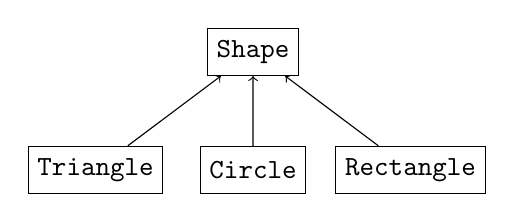
\begin{tikzpicture}[level 1/.style={sibling distance=20mm},minimum height=6mm]
\node (g1) [draw,->] {\tt Shape}
    child[<-]{node [draw] (s1) {\tt Triangle}}
    child[<-]{node [draw] (s2) {\tt Circle}}
    child[<-]{node [draw] (s3) {\tt Rectangle}};
\end{tikzpicture}
\end{center}
\vspace{2cm}

Куда добавить класс {\tt Square}?
\end{frame}

\begin{frame}[fragile]{Как правильно построить иерархию?}
    Квадрат — это прямоугольник, у которого все стороны равны.
\begin{center}
    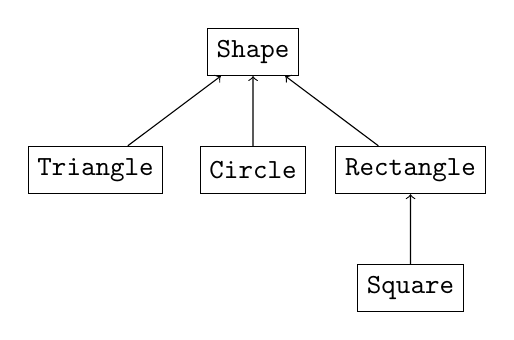
\begin{tikzpicture}[level 1/.style={sibling distance=20mm},minimum height=6mm]
\node (g1) [draw,->] {\tt Shape}
    child[<-]{node [draw] (s1) {\tt Triangle}}
    child[<-]{node [draw] (s2) {\tt Circle}}
    child[<-]{node [draw] (s3) {\tt Rectangle}
        child[<-]{node [draw] (s4) {\tt Square}}};
\end{tikzpicture}
\end{center}
\vspace{-2mm}
\begin{lstlisting}
void double_width(Rectangle & r) {
    r.set_width(r.width() * 2);
}
\end{lstlisting}
\end{frame}

\begin{frame}[fragile]{Как правильно построить иерархию?}
    Прямоугольник задаётся двумя сторонами, а квадрат — одной.
\begin{center}
    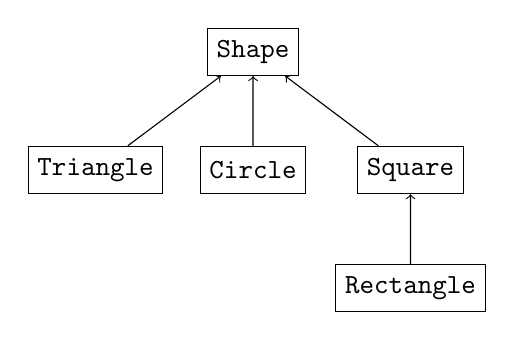
\begin{tikzpicture}[level 1/.style={sibling distance=20mm},minimum height=6mm]
\node (g1) [draw,->] {\tt Shape}
    child[<-]{node [draw] (s1) {\tt Triangle}}
    child[<-]{node [draw] (s2) {\tt Circle}}
    child[<-]{node [draw] (s3) {\tt Square}
        child[<-]{node [draw] (s4) {\tt Rectangle}}};
\end{tikzpicture}
\end{center}

\begin{lstlisting}
double area(Square const& s) {
    return s.width() * s.width();
}
\end{lstlisting}
\end{frame}

\begin{frame}[fragile]{Как правильно построить иерархию?}
    Правильное решение — сделать эти классы независимыми:
\begin{center}
    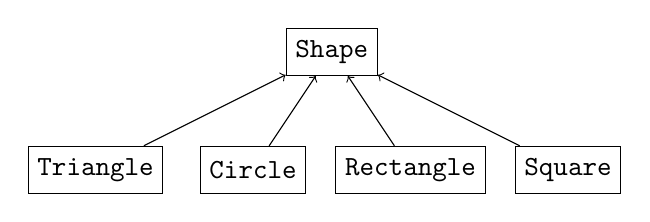
\begin{tikzpicture}[level 1/.style={sibling distance=20mm},minimum height=6mm]
\node (g1) [draw,->] {\tt Shape}
    child[<-]{node [draw] (s1) {\tt Triangle}}
    child[<-]{node [draw] (s2) {\tt Circle}}
    child[<-]{node [draw] (s3) {\tt Rectangle}}
    child[<-]{node [draw] (s4) {\tt Square}};
\end{tikzpicture}
\end{center}
\end{frame}

\begin{frame}[fragile]{Агрегирование vs наследование}
    \begin{itemize}
        \item {\em Агрегирование} — это включение объекта одного 
            класса в качестве поля в другой.

        \item Наследование устанавливает более сильные связи
            между классами, нежели агрегирование:
            \begin{itemize}
                \item приведение между объектами,
                \item доступ к {\tt protected} членам.
            \end{itemize}

        \item Если наследование можно заменить легко на агрегирование,
            то это нужно сделать.
    \end{itemize}
\begin{block}{Примеры некорректного наследования}
\begin{itemize}
    \item Класс {\tt Circle} унаследовать от класса {\tt Point}.
    \item Класс {\tt LinearSystem} унаследовать от класса {\tt Matrix}.
\end{itemize}
\end{block}
\end{frame}

\begin{frame}[fragile]{Принцип подстановки Барбары Лисков}
\begin{block}{Liskov Substitution Principle (LSP)} 
\em\centering  Функции, работающие с базовым классом, должны иметь 
    возможность работать с подклассами не зная об этом.
\end{block}
\vspace{5mm}
    
Этот принцип является важнейшим критерием при построении иерархий наследования. 

\begin{block}{Другие формулировки}
\begin{itemize}
    \item Поведение наследуемых классов не должно противоречить поведению,
            заданному базовым классом.
    \item Подкласс не должен требовать от вызывающего кода больше, чем базовый
        класс, и не должен предоставлять вызывающему коду меньше, чем базовый
        класс 
\end{itemize}
\end{block}
\end{frame}

\end{document}

 
